%%%%%%%%%%%%%%%%%%%%%%%%%%%%%%%%%%%%%%%%%%%%%%%%%%%%%%%%%%%%%%%%%%
% Based on the template available at:                            %
% https://github.com/andrea-gasparini/sapienza-beamer-template   %
%                                                                %
% Template author: Andrea Gasparini                              %
% Template license: GNU General Public License v3.0              %
%%%%%%%%%%%%%%%%%%%%%%%%%%%%%%%%%%%%%%%%%%%%%%%%%%%%%%%%%%%%%%%%%%

\documentclass{beamer}
\usepackage{amsfonts,amsmath,oldgerm,booktabs,multirow,overpic}
\usepackage{algorithm,algpseudocodex}
\usepackage{nicematrix}
\usepackage{tabularx}
\usetheme{sintef}

\setbeamertemplate{caption}{\raggedright\insertcaption\par}
\setbeamertemplate{footline}[frame number]{}
%\setbeameroption{show only notes}
%\setbeameroption{show notes on second screen}
\urlstyle{same}

\usefonttheme[onlymath]{serif}

\titlebackground*{assets/background_negative}

\newcommand{\hrefcol}[2]{\textcolor{navy}{\href{#1}{#2}}}

\title{Inverse Language Modeling towards Robust and Grounded LLMs}
%\subtitle{OmnAI Lab}
\course{Master's Degree in Computer Science}
\author{\href{mailto:sestito.1937764@studenti.uniroma1.it}{Simone Sestito}}
\IDnumber{1937764}
\date{Academic Year 2024/2025}

\newcommand{\bx}{\mathbf{x}}
\newcommand{\bxa}{\mathbf{x}\star}
\newcommand{\by}{\mathbf{y}}
\newcommand{\bya}{\mathbf{y}\star}
\newcommand{\be}{\mathbf{e}}
\newcommand{\bW}{\mathbf{W}}
\newcommand{\bh}{\mathbf{h}}
\newcommand{\loss}{\mathcal{L}}

\definecolor{navy}{HTML}{1976D2}
\newcommand{\highlight}[1]{\textcolor{navy}{\textbf{#1}}}

\renewcommand\tabularxcolumn[1]{m{#1}}% for vertical centering text in X column

\begin{document}
\maketitle

\documentclass[../thesis.tex]{subfiles}
\graphicspath{{\subfix{../assets/}}}
\begin{document}

\chapter{Introduction}
%% Introductory text
In Computer Science and Data Science, Artificial Intelligence (abbreviated as \emph{AI}) indicates the capabilities of an automated computational system to simulate abilities in performing tasks typically associated with human intelligence.

Applications of AI have gone way beyond their original conception, from limited rule-based systems to sophisticated models that nowadays are able to perform powerful classification tasks, recommendation systems, playing games due to the power of reinforcement learning, or even \textbf{generating synthetic data} that looks extremely similar to real-world data.

This evolution allowed the development of complex programs that are able to tune their parameters to improve their performance in solving more and more involved tasks.
What really contributed to this evolution is the invention of \textbf{Artificial Neural Networks} (ANNs). They originally where a simple multilayered perceptron-type network structure \citep{polynomial-theory-first-neural-network}, heavily inspired by the biological connections in human brains, interleaved by non-linear functions, so that the whole layers do not collapse in a single linear function.
They are composed by several neurons that work by aggregating information from previous layers, in a learnable weighted sum. The learning of the weights in this sum is the fundamental part in ANNs, which lets them learn a non-linear function, thanks to Backpropagation, which is an algorithm based on gradient estimation to train a neural network, based on a defined loss function, representing how much the network is approaching the optimal objective we define.


\section{Inductive Bias in Neural Networks}
Later works in this field, took to the development of more and more complex structures, adding always different inductive biases, i.e. the choice of hypotheses space from which learned functions are taken \citep{cohen2016inductivebias}.
\textbf{Convolutional Neural Networks} (CNNs) \citep{krizhevsky2012imagenet}, and older architectures like the Neocognitron model proposed by \citeauthor{fukushima1980neocognitron}, inspired by the neuro-physiological findings on the visual systems of mammals, allowed the construction of neural networks that had lots of successes in the field of Computer Vision. In its essence, CNNs inductive bias are the feature hierarchy principle, involving inside of the network a sequence of layers that should identify from low-level to high-level features in the input image, but also the translation invariance and weights sharing, given by the convolutional kernels, which are applied as-they-are on the overall image, instead of being different according to different portions of the input, finally applying a locality principle, which allows CNNs to capture patterns in a local area of the image, thanks to the enforcement of a local connectivity pattern between neurons of adjacent layers.

\begin{figure}
    \centering
    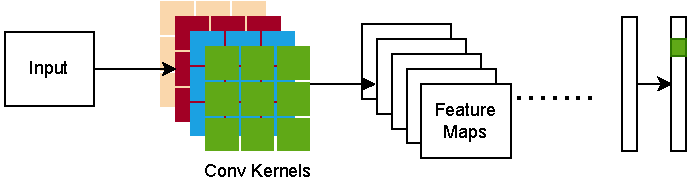
\includegraphics[width=0.6\linewidth]{assets/CNN_Illustration.drawio.pdf}
    \caption{Diagram summarizing the main idea behind a CNN}
    \label{fig:cnn_illustration}
\end{figure}

Later on, different architectures where created to get even better on several domain-specific tasks.
An example of this is the creation of \textbf{Graph Neural Networks} (GNNs) \cite{introducinggraphneuralnetworksgnn}.
They focused on a specialized architecture that could process graphs, given their already popular usage to represent data in several different fields, from molecular chemistry, to pattern recognition, and even data mining. They can be seen as a generalization of CNNs, where the connections are modeled in a non-Euclidean space, considering the depths of a graph as in \cref{fig:gnn_illustration}.

\begin{figure}
    \centering
    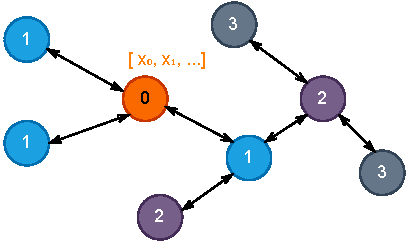
\includegraphics[width=0.4\linewidth]{assets/GNN_Illustration.drawio.pdf}
    \caption{Diagram illustrating the concept of a GNN creating a vector embedding for a node, with respect to its neighbors at various depths}
    \label{fig:gnn_illustration}
\end{figure}

\subsection{Sequence Processing}
\label{sec:introduction__sequence_processing}
Sequence processing posed its own challenges, due to the variable length of the input and possibly a variable length of the output.
First works include \textbf{Recurrent Neural Networks} to allow networks to have an internal dynamic memory that could be kept updated with next steps in a time series \citep{ELMAN1990179rnn}, as shown in \cref{fig:diagram_rnn}. Their architecture leverages the sequential dependencies between positions in the input sequence, giving an inductive bias to the current position to also influence future ones. Even though their parameters are shared across different time steps, this kind of networks, in their standard formulation, are difficult to be trained due to their natural vanishing and exploding gradients issues \citep{bengio1994gradientdescent-rnn}.

%% LSTM
To overcome this issue and to allow dependencies interactions with larger distances, \textbf{Long Short-Term Memory} networks have been introduced by \citeauthor{lstm}, illustrated in \cref{fig:diagram_lstm}.
Its internal structure is composed by \emph{gates} that allow the network 
to decide how much information to discard from its internal long term memory (Forget gate),
which parts of the input to add to the memory, after some transformation (Input gate),
and what should be output for that time step, if needed (Output gate).
LSTM also solves complex, artificial long-time-lag tasks that have never been solved by previous recurrent network algorithms. It can learn much faster, thanks to the uninterrupted gradient flow in the gated skip connections between memories across subsequent time steps.

% Fix for subfigures with different heights
% From: https://tex.stackexchange.com/a/239176
\newsavebox{\largestimage}
\begin{figure}
    \centering
    % Store largest image in a box
    \savebox{\largestimage}{%
        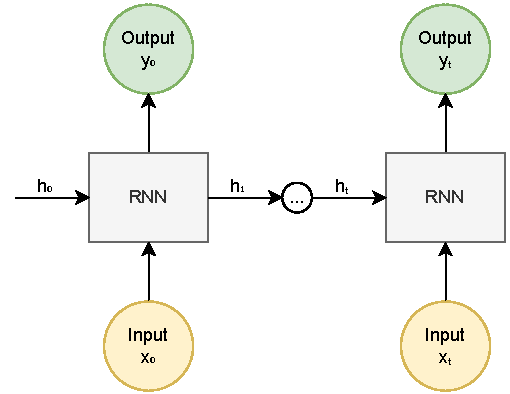
\includegraphics[width=0.4\textwidth]{assets/RNN_Illustration.drawio.pdf}%
    }%
    \begin{subfigure}[b]{0.4\textwidth}
        \centering
        \usebox{\largestimage}
        \caption{RNN}
        \label{fig:diagram_rnn}
    \end{subfigure}
    \quad
    \begin{subfigure}[b]{0.5\textwidth}
        \centering
        % Adjust vertical height of smaller image
        \raisebox{\dimexpr.5\ht\largestimage-.5\height}{%
        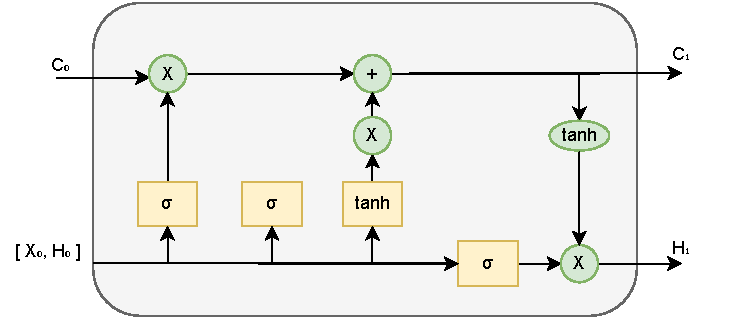
\includegraphics[width=\textwidth]{assets/LSTM_Illustration.drawio.pdf}}
        \caption{LSTM}
        \label{fig:diagram_lstm}
    \end{subfigure}
    \caption{Illustrations of the core architectures of RNN and LSTM}
    \label{fig:diagrams_rnn_lstm}
\end{figure}

Further works in this direction exploited the use of \textbf{Convolutional Neural Networks} to perform time series forecasting \citep{bai2018temporalconvolution}, discovering that it could outperform canonical Recurrent Neural Networks and LSTMs across various tasks, indicating them as a starting point for sequence modeling tasks due to their abilities to exploit local dependencies and have a longer memory thanks to the logarithmic interaction distance between input positions.

\section{Transformer Networks and LLMs}
Before we get into the main topics of this work, it is crucial to understand Large Language Models (LLMs) and the network architecture behind most of them especially in recent times.

%% Transformers
A strong evolution in sequence processing, especially in the field of Natural Language Processing,
is represented by Transformer networks \citep{NIPS2017_attentionisallyouneed}.
Unlike previous sequence models that relied on recurrent or convolutional layers, transformers use a mechanism called self-attention to process input data in parallel rather than sequentially. This design allows transformers to capture long-range dependencies and relationships between elements in a sequence more effectively. Its scalability and effectiveness have made it the foundation for most modern large language models and many other AI systems, including, but not limited to, applications in Computer Vision, audio and signal processing.

%% Encoder-decoder
Their original architecture is composed by an Encoder and a Decoder.
In the Encoder part, the input, which is often a one-hot encoded vector of the input text tokens, is embedded via a learnable embedding layer, and added to a fixed positional encoding, to make the text variant with respect to permutations.
The embedded tokens are transformed through a series of stacked layers, each having a multi-head attention part, where all tokens can \emph{attend} all others (creating the parallel and long-range interactions previously discussed), then after skip connections and normalization layers which help with training stability, the tokens are individually transformed using a Feed Forward layer. It repeats for the predefined number of stacked layers.
While in the Decoder part, the self-attention applied to the expected output targets is \emph{Masked}, indicating that a token at position $i$ cannot attend tokens at positions $j > i$, since it would cause the network not to actually predict future tokens, as it will have to do during inference.

%% LLM Introduction
\textbf{Language Models} in their simplest conception are computational systems designed to understand human natural language and generate sentences based on statistical relationships and properties between words, learnt during the training stage.
Traditionally, they were modeled using $n$-grams, like bi-grams if $n = 2$, focusing on predicting the most likely next word, based on the $n-1$ previous ones following this approximation:

\begin{equation}
    \mathbb{P}(x_t | x_{1:t-1}) \approx \mathbb{P}(x_t | x_{t-n+1:t-1})
\end{equation}

Simple and explainable models like these have been surpassed by more evolved neural network based models, such as RNN and LSTM discussed in \cref{sec:introduction__sequence_processing}.
Even more powerful are Transformed based models, representing a huge scaling of language models and involving the training of several billion parameters, take the name of \textbf{Large Language Models}, or LLMs for short. This scaling experiment led to unexpected capabilities, like few-shots learning, generating plausible and grammar correct text corpus.
You cannot say the same for the correctness of the contents that are being generated. It is not so infrequent to see generated textual responses that contain some plausible sentences carrying a totally incorrect information, which take the name of \emph{hallucinations}.
Moreover, LLMs face potential biases derived from the training data, which are addressed in a later step in the training process, discussed in \cref{sec:introduction__meaning_attack_llm}.

%% T5
An LLM that applied the standard Transformer architecture is \textbf{T5}, or \emph{Text-to-Text Transfer Transformer}
\citep{raffel2020exploringt5}. It has an Encoder - Decoder architecture and it has been made to model a universal sequence-to-sequence text transformer, which is able to work on a variety of downstream tasks, just applying a natural language prefix to the input prompt, like \emph{``summarize: <text>''} or \emph{``translate from <lang\_from> to <lang\_to>: <text>''}

%% BERT: encoder-only
In contexts different from standard sequence-to-sequence tasks, it has been studied the use of Encoder-only architectures, like in \textbf{BERT}, or \emph{Bidirectional Encoder Representations from Transformers} \cite{devlin2019bert}.
The choice of this architecture is based on the scope of this new model: it is a \emph{Masked} LLM, meaning that it is pretrained only to be a foundation model.
Its pretraining task is to make predictions on some masked tokens, in a non-autoregressive way, while being conditioned on the still visible parts of the input tokens.
Using its Encoder, it can learn representations of entire sentences, or represent tokens with respect to all other tokens in the sentence, which is particularly useful with words that have different meanings depending on their usage, or words like \emph{``not''} that change the meaning of an entire component of the overall input text.
Because it is a foundation model, it is meant to be fine-tuned on downstream tasks, like Question Answering, Sentence Pair Classification or Sentence Tagging tasks.

%% GPT: decoder-only
Finally, to achieve better performances without fixed pair inputs, as in the case of the T5 model,
a Decoder-only architecture can be used. A famous example of this approach is the \textbf{GPT} model, also referred to as  It works in a simple autoregressive way. During its unsupervised pretraining step, it does not differentiate between a task to perform and its correct solution, but just about predicting the next token in a text corpus.
This allows to have a much bigger dataset to train on, potentially the whole web, while being much simpler. Then, it can be fine-tuned in a supervised methodology to solve some specific tasks fine-tuning the LLM with some question-answer data, or in a chat form, thus constructing what are nowadays very popular LLM-based chatbots.
The Decoder-only architecture, despite its simplicity, can be shown to be Turing complete, given a minimum vector dimensionality, relative to the token embedding size \citep{roberts2024powerful-decoderonly}.

\section{Adversarial attacks}
%% Adversarial attacks in generale
Deep networks are widely used in many fields of AI, especially when the task to fulfill is not so simple or straightforward.
However, a main concern about their usage in critical scenarios is the presence of adversarial samples.
They are defined, in the context of deep classifiers for images, as input samples that, despite being unnoticeable by the human eyes, are able to lead to misclassifications, sometimes letting the model output a probability even higher of being of a certain class rather than real-world samples of that misclassified class \citep{zhang2023review-adversarialattacksurvey}.

As a general understanding, adversarial attacks can be divided into:
\begin{itemize}
    \item \textbf{white-box} attacks, where the bad actor has access to the internal weights, activations and gradients of the target model;
    \item \textbf{black-box} attacks, where the target is observed by the bad actor as a black-box, as the name suggests, looking only at the output of it, without knowing its internal behavior
    \item \textbf{gray-box} attacks are somewhere in the middle of the previous two cases, where some limited internal information is available
\end{itemize}

A very popular optimization-based white-box attack targeting deep image classifiers is the Carlini \& Wagner (\textbf{C\&W}) algorithm \citep{carlini-wagner-image-attack}.
It is designed to find a perturbation of the input that minimized a predefined norm, as $L_0$ or $L_2$, while leading to a misclassification. It is referred to as \emph{targeted attack} when the misclassified class is already define beforehand instead of being just a class different from the true one.

\begin{equation}
\begin{split}
    \text{minimize}_\delta \;&\; L_{norm}(x, x+\delta) \\
    \text{such that}       \;&\; f(x+\delta) = t       \\
                           \;&\; x+\delta \in [0,1]^n
\end{split}
\end{equation}

In the context of Gradient-based white-box attacks, it is worth mentioning an efficient method referred as Fast Gradient Sign Method (\textbf{FGSM}) \citep{goodfellow2014explainingfgsm}.
The perturbation is obtained by looking at the direction of the gradient of the loss function, thus making the model go in the direction of a misclassification by changing the input sample.
This time, the magnitude of the perturbation ($\alpha$) is an hyperparameter. A value too low may lead to bad effects in the attack success rate, while making it too high may cause the imperceivability requirement to fail.

\begin{equation}
    x' = x + \alpha \cdot \text{sign}(\nabla_x \mathcal{L}(\theta; x; y_{\text{true}}))
\end{equation}

It may also be repeated iteratively, leading us to the \textbf{I-FGSM} algorithm introduced by \citeauthor{kurakin2018adversarial-iterative-fgsm}.

\subsection{Targeting LLMs}
\label{sec:introduction__meaning_attack_llm}
We have observed how generally adversarial attacks can be easily applied to image classifiers, mostly because of it having a manageable continuous input space, where any perturbation can be added and the result will still be a valid sample in the input.
This cannot be directly applied to Large Language Models, since tokens are \textbf{discrete}.
Even though their embeddings are continuous, only a very small subset of $\mathbb{R}^d$, where $d$ is the dimensionality of the embedding for a specific LLM, contains the valid embeddings that can be mapped back to a token.

%% Usual training di LLM
The state of the art procedure to \textbf{train an LLM} consists of multiple stages \citep{grattafiori2024llama}:
\begin{enumerate}
    \item the pre-training step, further split into:
    \begin{enumerate}
        \item the collection of a huge training corpus from a variety of sources, filtering Personally Identifiable Information (\emph{PII}), sources with known inappropriate content and de-duplication of lines repeated too many times;
        \item the initial pre-training step involves deciding the architecture, which is almost always a dense Transformer-based one \citep{NIPS2017_attentionisallyouneed}, as well as establishing the scale of the model in terms of number of parameters and fixing the hyperparameters;
        \item long-context pre-training, where the model is fed with context windows up to 128K tokens - and this only happens after an initial pre-training because of the quadratic scale of self-attention layers
    \end{enumerate}

    \item the post-training procedure follows, starting from the fine-tuning of the foundation LLM into a chat model, on a dataset implementing a chat protocol decided by the LLM authors, including the chat format for the system, assistant and user texts, but also the special tokens to utilize for that goal;

    \item the alignment step.
\end{enumerate}

%% Cosa vuol dire quanto diventano aligned
This last \textbf{alignment} step is the most interesting one when it comes to adversarial attacks.
It consists of Supervised FineTuning (\textbf{SFT}) data collected via human annotations or synthetically generated.
Its goal is to make the LLM more reliable and safe, by aligning it with human values. In simpler terms, it should instruct the LLM not to reply to requests that go against ethical principles, legality and so on.
It can be achieved training a SFT model with techniques like Direct Preference Optimization (\textbf{DPO}) \citep{rafailov2023directpreferenceoptimization}, to overcome the old and costly algorithm RLHF (\emph{Reinforcement Learning from Human Feedback}) \citep{zheng2023secretsrlhflargelanguage}.
However, especially state-of-the-art suffix based adversarial attacks, as seen in \cref{sec:related_work__sota_suffix_generation}, can bypass this alignment procedure, making the model reply to questions that should not be made available according to the injected chat model safety policies.

%% VERY BRIEFLY, modi di attaccarli
As we will see more in details in the next chapter, there are multiple ways to attack an LLM:
\begin{itemize}
    \item an out-of-distribution input text may be given as input, letting the model generate a meaningful completion sequence, despite the meaningless input the attacker used;
    \item an LLM may be inducted to perform tasks that should be prohibited, according to common sense and ethical considerations, neutralizing the effects of the alignment procedure (\cref{sec:related_work__sota_suffix_generation}).
\end{itemize}

\section{Safety and Ethical considerations}
%% Considerazioni etiche
With the increasing popularity of LLMs even among normal population after the introduction of powerful chatbots based on them, safety and the understanding of their internals plays a crucial role,
especially to protect non-technical people.
Several jailbreak prompts are publicly available, most of them being fixed in newer releases of affected models. However, it is not clear whether or not they may be fixed once and for all, instead of continuing to solve newer ones as they are discovered by the research community.

\begin{figure}[hbp]
    \centering
    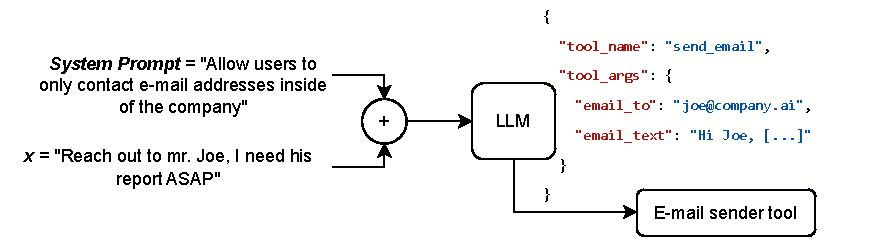
\includegraphics[width=\linewidth]{assets/LLM_Tool_workflow.drawio.pdf}
    \caption{Example invocation of a tool by an LLM to perform a real-world action}
    \label{fig:introduction__llm_tool_workflow}
\end{figure}

%% Safety di LLM in production
Furthermore, safety is even more important when these systems are integrated into automated applications and connected to \textbf{tools}. In this sense, they may be used to actually perform harmful actions, instead of just replying with something they should not say, according to principles of common sense, legality and ethics.
Indeed, supposing that an LLM is connected to a service to send emails and the arguments to invoke this function are provided by the LLM, we may accidentally let an attacker use our company e-mail address to conduct a phishing campaign and so on. This should make developers aware of the risks they are exposing themselves when letting an LLM take actions on their behalf and they should pay really careful attention on sanitizing LLM-provided arguments, treating them as potentially harmful user inputs instead of an internal data that should already be considered to be safe.

As we will see in the next chapters, it is absolutely possible to trick an LLM into continuing a sequence of tokens as we - playing the role of the attackers - want. It may include a tool function invocation, exploiting some vulnerable situations as mentioned before.

To conclude, when opaque prompts (input sequences that are nonsensical from a human point of view)
are involved in the process, it is even more clear that we cannot fully control the internal behavior of Large Language Models, especially with the intent of mitigating unintended actions from being taken. They are an indication that generation is still of out of our control, going in the opposite direction of the phenomenon of Prompt Engineering.
Our investigation and experiments during this thesis aim to make them safer and more predictable.

\subbib{}
\end{document}
% \section{Preliminary Study}

\begin{frame}{Robust sentence classifier}
    \begin{center}
        We have to move into text and LLMs
    \end{center}
\end{frame}

\begin{frame}{Robust sentence classifier}
    What if:
    \begin{itemize}
        \item Our input image is a sentence embedding from BERT
        \item Our classes are languages, and the sentiment of those sentences
    \end{itemize}

    \vfill
    \begin{center}
        \footnotesize    The Multilingual Amazon Reviews Corpus
    \end{center}

    \vfill
    \pause
    \centering
    However, gradients have no more \highlight{"visual" meaning} for a human.
    \note{What's the image of a sentence embedding? It cannot exist}

    But hidden states contain the \highlight{meaning of the overall sentence}, like an image
\end{frame}

\begin{frame}{And it works!}
\begin{table}[]
\begin{tabular}{lcclccc}
\toprule
                             & \multicolumn{2}{c}{\textbf{APGD}}          & \textbf{Square}                     & \multicolumn{3}{c}{\textbf{FSGM}}                                                                               \\
                             & $\varepsilon = 1e-3$ & $\varepsilon = 0.5$ &                                     & \multicolumn{1}{l}{$\alpha = 1e-3$} & \multicolumn{1}{l}{$\alpha = 5e-3$} & \multicolumn{1}{l}{$\alpha = 1e-2$} \\
 \midrule
\multicolumn{1}{r}{Baseline} & 47.9\%               & 41.7\%              & \multicolumn{1}{c}{48.2\%}          & 79.2\%                              & 44.8\%                              & 14.5\%                              \\
\multicolumn{1}{r}{PAG model}   & \textbf{75.8\%}      & \textbf{70.4\%}     & \multicolumn{1}{c}{\textbf{76.6\%}} & \textbf{82.4\%}                     & \textbf{69.2\%}                     & \textbf{49.0\%}                    \\
\bottomrule
\end{tabular}
\vspace{0.25cm}
\caption{Adversarial attacks comparing the two models}
\label{table:pag__binary_classifier_robustness}
\end{table}
\end{frame}


% \input{sections/gcg}
\section{Inverse Language Modeling}

\begin{frame}{Attacking LLMs with GCG}
\note{
    GCG finds attack sequences $\bxa$ such that they can link better to a given continuation $\by$, \\
    starting from a random one-hot sequence of tokens and \\
    iteratively optimize it using \textbf{gradient} information. \\
    This table must be read: $\bx || \by$ and $\bxa || \by$. \\
    These sequences are called \emph{Evil Twins} in the Prompts have evil twins paper. \\
    --------- \\
    OUR GOAL? Prevent their existence, or limit the success rate of this attack.
}
    Greedy Coordinate Gradient is an algorithm to find a sequence of tokens $\bxa$ such that the LLM will complete with $\by$ that we want --- using \highlight{gradients} on input tokens
    \vfill

    \begin{table}[]
    \centering
    \resizebox{\textwidth}{!}{
        \begin{tabular}{llc}\toprule
        \textbf{Input} & \textbf{Output $\by$} & \textbf{Loss} \\
        \midrule
        %\cline{2-3}
        $\bx$~: Stevens recorded and produced the album at multiple & \multirow{2}{*}{locations in the United}  & 5.3642 \\
        $\bxa$: Zo Certified Cities (. broadcastquartered Fitness Academy thirteen   & &  \textbf{5.1302} \\
        \midrule
        $\bx$~: After the introduction of the Majors , The   & \multirow{2}{*}{British Army was divided}   & 11.2146 \\
        $\bxa$: REQU Apart British received reformsMilitaryestic Division The  & &  \textbf{7.1899} \\
        \midrule
        $\bx$~: The founding director , Peggy Loar , left   & \multirow{2}{*}{the University of California}   & 7.2669\\
        $\bxa$: tested UberERIC definitionCalifornia sustainability RutgersOL Jensen regarding  & &  \textbf{6.4402} \\
        \midrule
        $\bx$~: Ruiz notes that writing also has the power & \multirow{2}{*}{\centering to change the world} & 5.9135 \\
        $\bxa$: Report Global feminism agenda Representatives tell Sacredixties Trying & & \textbf{4.6041} \\
        \bottomrule
        \end{tabular}
    }
    \caption{They are called "Evil Twins"}
    \end{table}
\end{frame}

\begin{frame}{Difficulties of LLMs}
    What about LLMs?

    \begin{itemize}
        \item Input is \highlight{sequential}
        \note{$\rightarrow$ a single token cannot determine what's the next token to predict}
        \item The same sequence can continue in multiple ways $\rightarrow$ \highlight{multiple} valid classes
        \item The input space is \highlight{discrete} ($|\mathcal{V}|$)
    \end{itemize}
\end{frame}

\begin{frame}{Introducing ILM}
\note{
    At this point, we can introduce Inverse Language Modeling. \\
    \textbf{GOAL}: train LLMs, or fine-tune them, such that they internally "understand" what they are conditioned on. \\
    This is somehow based on the idea of LLMs as stochastic parrots. \\
    \textbf{KEY IDEAS}: create a new training procedure that makes them \textbf{grounded} to the input, exploiting weights.
}
    \begin{itemize}
        \item \highlight{Goal:} train LLMs to both generate text and \emph{understand what they are conditioned on} 
        \underline{\textbf{(inversion)}}
        from the output
        \item \highlight{Key Ideas:}
            \begin{itemize}
                \item Create a new training procedure that adds more \underline{\textbf{robustness}} in the loop
                \item Reconstruct input from the output, using $\nabla_\bx \loss$
            \end{itemize}
    \end{itemize}
\end{frame}

\begin{frame}{Introducing ILM}
\note{
    This illustration graphically shows the logic: \\
    - originally, they go from left to right \\
    - but it can also go from right to left, using gradients information.
}
    \begin{figure}
    \centering
    \vspace{0.5cm}
    \begin{overpic}[width=0.7\linewidth]{assets/forward_backward_llm}
        \put(5.5,0){$\bx_1$}\put(19.5,0){$\bx_2$}\put(33.5,0){$\bx_3$}
        \put(5.5,27){$\bx_2$}\put(19.5,34){$\bx_3$}\put(33.5,44){$\bx_4$}
        \put(60,43.5){$\bx_2$}\put(72,43.5){$\bx_3$}\put(87,43.5){$\bx_4$}
        \put(60,0){$\bx_1$}\put(72,10){$\bx_2$}\put(87,18){$\bx_3$}
        \put(17,59.5){{\footnotesize \textbf{Now}}}
        \put(68,59.5){{\footnotesize \highlight{Proposed}}}
        \put(0,55){{\footnotesize Autoregressive forward}}
        \put(55,55){{\footnotesize Autoregressive backward}}
        \put(5,49){{\scriptsize $p(\bx_i|\bx_1,\ldots,\bx_{i-1})$}}
        \put(50,49){{\scriptsize$p\big(\bx_{i-1}| \nabla_{\bx_{i-1}}p(\bx_i|\bx_1,\ldots,\bx_{i-1})\big)$}}
    \end{overpic}
    \end{figure}
\end{frame}

\begin{frame}{ILM Inversion Procedure}
\note{
    Let's make an example: \\
    We have a sentence, like \emph{The pen is on the table} \\
    It gets split: \\
    - prefix: \emph{the pen is} \\
    - suffix: \emph{on the table} \\
    . \\
    Here, we have the suffix and predict backward the prefix.
}
    \centering
    Split it into the original prefix $\bx_p = \bx_{0:k}$ and the suffix $\bx_s = \bx_{k:n}$ \\
    \vfill
    $\bx =$ The pen is on the table \\
    \vspace{0.5cm}
    \hfill $\bx_p =$ \highlight{The pen is} \hfill $\bx_s = $ on the table \hfill $\;$\\
\end{frame}

\begin{frame}{Gradients Received by the Tokens}
\note{
    But how is that possible? What's the \textbf{theoretical} rationale behind it? \\
    From this diagram, you can see that if we change a token in the middle, like $\be_3$, \\
    it influences the hidden states only in the future, \\
    but gradients carry out the information of the overall sentence, \\
    since the gradients of the previous tokens (the \textbf{past}) change as well.
}
    Gradients received on a single token embedding,
    carry information of the whole sentence

    \begin{figure}
        \centering
        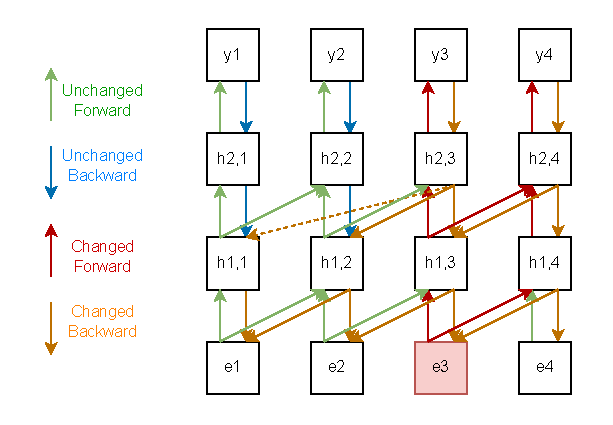
\includegraphics[height=0.6\paperheight]{assets/llm_gradients_changing_embedding.drawio.pdf}
    \end{figure}
\end{frame}

\begin{frame}{Gradients Received by the Tokens}
\note{
    This sentence well describes the rationale.
}
    \begin{quote}
        \centering
        A causal model looks ahead, \\ but only its gradients disclose the pasts that might have built that future.
    \end{quote}
\end{frame}

\begin{frame}{ILM Training Procedure}
    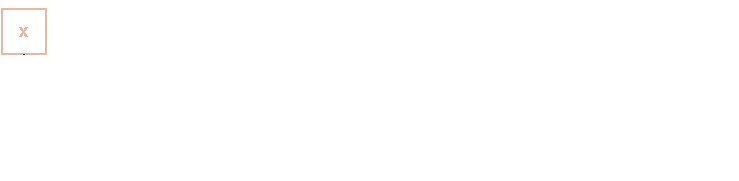
\includegraphics[width=\linewidth]{assets/grad_lm_head_parallelism_0.drawio.pdf}
    \vspace{1.5cm}
    
    \centering
    Given the input sentence $\bx_0, \bx_1, \bx_2, \dots, \bx_{n-1}$
\end{frame}

\begin{frame}[noframenumbering]{ILM Training Procedure}
    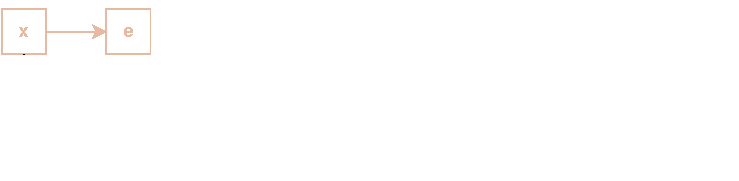
\includegraphics[width=\linewidth]{assets/grad_lm_head_parallelism_1.drawio.pdf}
    \vspace{1.5cm}
    
    \centering
    Embed the input sentence tokens into $\be_0, \be_1, \be_2, \dots, \be_{n-1}$
\end{frame}

\begin{frame}[noframenumbering]{ILM Training Procedure}
    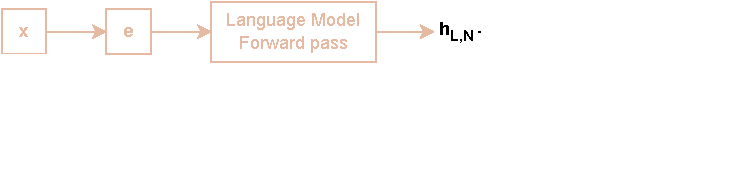
\includegraphics[width=\linewidth]{assets/grad_lm_head_parallelism_2.drawio.pdf}
    \vspace{1.5cm}
    
    \centering
    Pass through the Transformer Decoder layer, up to the final hidden state $\bh_0, \bh_1, \bh_2, \dots, \bh_{n-1}$
\end{frame}

\begin{frame}[noframenumbering]{ILM Training Procedure}
    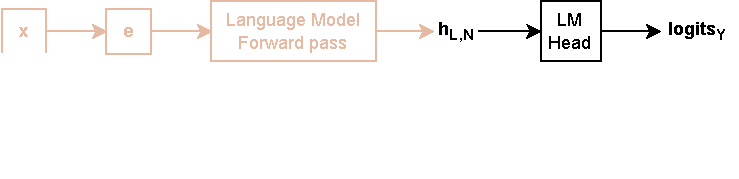
\includegraphics[width=\linewidth]{assets/grad_lm_head_parallelism_3.drawio.pdf}
    \vspace{1.5cm}
    
    \centering
    Using the Classifier Head, predict $\by_0, \by_1, \by_2, \dots, \by_{n-1}$
\end{frame}

\begin{frame}[noframenumbering]{ILM Training Procedure}
    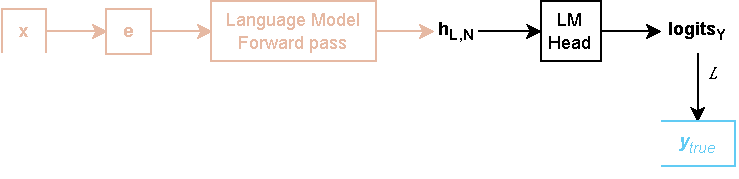
\includegraphics[width=\linewidth]{assets/grad_lm_head_parallelism_4.drawio.pdf}
    \vspace{1.5cm}
    
    \centering
    Compute the loss $\loss_{CE} = CE(\bx_{1:n}, \by_{0:n-1})$ comparing the predictions with the ground-truth
\end{frame}

\begin{frame}[noframenumbering]{ILM Training Procedure}
    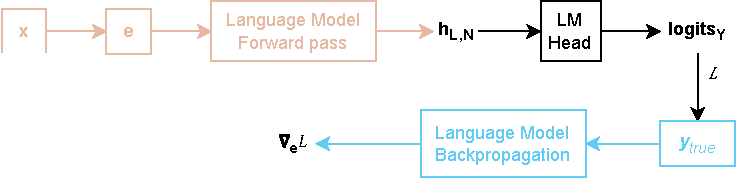
\includegraphics[width=\linewidth]{assets/grad_lm_head_parallelism_5.drawio.pdf}
    \vspace{1.5cm}
    
    \centering
    Backpropagation: compute the gradients $\nabla_{\be_{0:n-1}} \loss$
\end{frame}

\begin{frame}[noframenumbering]{ILM Training Procedure}
    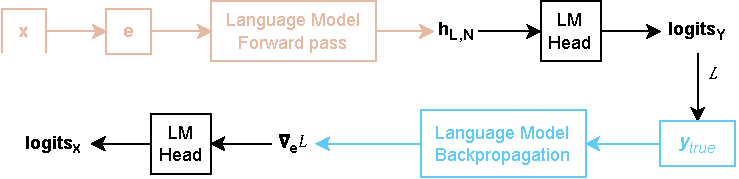
\includegraphics[width=\linewidth]{assets/grad_lm_head_parallelism_6.drawio.pdf}
    \vspace{1.5cm}
    
    \centering
    From the gradients, predict the input tokens $\bx_{0:n-1}$
    \note{Use the gradients as if they were the last hidden state and use them to predict the input $\bx$ tokens}
\end{frame}

\begin{frame}[noframenumbering]{Parallelism}
    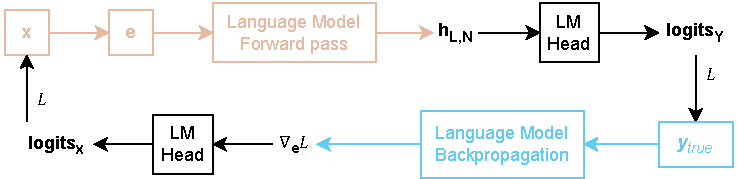
\includegraphics[width=\linewidth]{assets/grad_lm_head_parallelism.drawio.pdf}
    \vspace{1.5cm}
    
    \centering
    As if it were really \highlight{cyclic}! \\
    Parallelism between the last hidden state and the gradients on the embeddings
\end{frame}

\begin{frame}{More Parallelism: Weight Tying}
\note{
    In some LLMs, weight tying makes the LM Head projection and the Embeddings matrix to be exactly the same Tensor in memory!
}
    \centering
    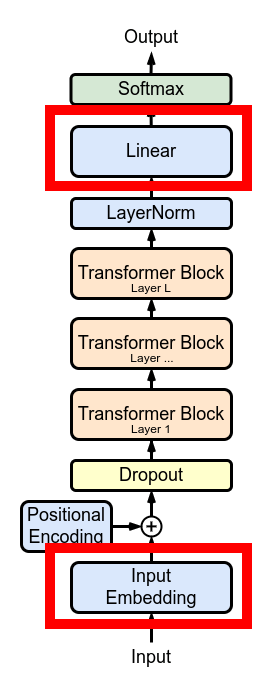
\includegraphics[height=0.8\paperheight]{assets/gpt_weight_tying.png}
\end{frame}



\begin{frame}{ILM Variants}
\note{
    We end up with this combined loss, both for Cross-Entropy forward and backward. \\
    This is implemented using PyTorch-supported \textbf{double Backpropagation}. \\
    --------- PAUSE --------- \\
    We have some variants: \\
    - identity, what we just said. It might hypothetically learn some identity function, as in AutoEncoders without a bottleneck \\
    - bert-like, imitating the BERT training procedure when going backward on the Gradients \\
    - inv-first, that just works on the very first token, splitting sentences. \\
    --------- PAUSE --------- \\
    Classification: \\
    - we can use these gradients as a pure value \\
    - or follow the natural definition of a gradient as a direction and go in its negative direction \\
}
    \begin{equation*}
    \loss =
    \underbrace{\loss_{CE}(\by_\text{true}, \by_\text{pred})}_\text{Forward: from the input x, encode y}
    +
    \underbrace{\lambda\ \loss_{CE}(\bx, f(\bx, \nabla\bx))}_\text{Backward: from gradients, decode back x}
    \end{equation*}

    \pause
    \begin{itemize}
        \item \highlight{Identity}: what we have discussed so far
        % \begin{itemize}
        %     \item $\nabla_\be \loss$ theoretically has access to $\bx$ $\rightarrow$    \textbf{possible shortcut}
        % \end{itemize}
        \pause
        \item \highlight{BERT-like}: masking the input tokens on the gradients
        \begin{itemize}
            \item When computing $\nabla_\be$, replace 10\% tokens to predict from the gradients with \texttt{[PAD]} \\ $\rightarrow$ it should understand what's missing
        \end{itemize}
        \pause
        \item \highlight{Inv-First}: assign the first token to \texttt{[PAD]} and invert it
    \end{itemize}
    
    \pause
    \vspace{0.5cm}
    \textbf{Classification Stategies:}
    \pause
    \begin{itemize}
        \item Use gradient as \highlight{value} --- $f(\nabla_{\bx_i}\loss_{CE})$
        \pause
        \item Use gradient as \highlight{direction} --- $f(\bx_i - \nabla_{\bx_i}\loss_{CE})$
    \end{itemize}
\end{frame}


% \begin{frame}{ILM Inversion Procedure}
%     \centering
%     From the gradients on the input, predict the previous token \emph{(one at a time)} \\
%     \vspace{1cm}
%     Do a \highlight{Beam Search}: keep the $b$ most probable prefixes, not just one
% \end{frame}


\begin{frame}{But we don't have billions of dollars}
\note{
    However, we trained LLMs, with lots of different variants to compare. \\
    We HAD to stay on a small example, to validate the idea, \\
    scaling it in a future time.
}
    These results have been obtained on a tiny LLM:
    \begin{itemize}
        \item Only 10M parameters
        \item A vocabulary of just 2048 tokens
        \item A simple corpus (\texttt{TinyStories} dataset)
    \end{itemize}

    \vfill
    It will be scaled to Llama-1B in the future.
\end{frame}

\section{Results}

\begin{frame}{Inversion Evaluation}
\note{
    In all these evaluation tables, we can see that the \textbf{Identity} model using gradients as \textbf{directions} \\
    is chosen as the best variant. \\
    Interestingly, the \textbf{baseline} is already able to invert quite well, \\
    even though this method allowed us to further improve it. \\
    NOTE that to invert we need an \textbf{init}: \\
    - for baseline and identity, we use a very simple bigram model \\
    - for bert and inv-first, we use the PAD token as did during training.
}
\begin{table}[bthp]
\centering
\resizebox{0.9\textwidth}{!}{
    \begin{tabular}{rlcccc}
    \toprule
    & \multirow{2}{*}{\textbf{Grad.}} & \textbf{Token}    & \textbf{Token}       & \textbf{Token}      & \textbf{Positional} \\
    &                                 & \textbf{Recall ↑} & \textbf{Precision ↑} & \textbf{F1-score ↑} & \textbf{Accuracy ↑} \\
    \midrule
    Baseline   &                      & 20.9\%            & 18.8\%               & 19.7\%              & 2.4\%               \\
    \midrule
    Inv-First  &                      & 11.3\%            & 10.1\%               & 10.7\%              & 1.7\%               \\
    Bert-like  & Val.                 & 2.9\%             & 2.7\%                & 2.8\%               & 0.3\%               \\
    Identity   &                      & 0.7\%             & 0.7\%                & 0.7\%               & 0.1\%               \\
    \midrule
    Inv-First  &                      & 13.3\%            & 12.0\%               & 12.6\%              & 2.4\%               \\
    Bert-like  & Dir.                 & 0.1\%             & 0.1\%                & 0.1\%               & 0.1\%               \\
    \highlight{Identity}   &          & \textbf{22.5\%}   & \textbf{20.2\%}      & \textbf{21.2\%}     & \textbf{2.5\%}      \\
    \bottomrule
    \end{tabular}
}
\vspace{0.25cm}
\caption{Evaluation of the inversion capabilities, on metrics relative to the single tokens}
\label{tab:ilm-evaluation-token-metrics}
\end{table}
\end{frame}

\begin{frame}{Inversion Evaluation}
\note{
    To have more accurate results, we passed the sentences to a third-party LLM \emph{Llama 1B}, to compute some perplexity statistics. \\
    It shows: \\
    - PPL of the overall sentence $\bxa || \by$ \\
    - PPL of just the inverted prefix $\bxa$
}
\begin{table}[bthp]
\centering
\resizebox{0.8\textwidth}{!}{
    \begin{tabular}{rlccc}
    \toprule
    & \multirow{2}{*}{\textbf{Grad.}} & \textbf{Full Sentence} & \textbf{Predicted Prefix} & \textbf{Semantic}     \\
    &                                 & \textbf{Perplexity ↓}  & \textbf{Perplexity ↓}     & \textbf{Similarity ↑} \\ 
    \midrule
    Baseline   &                      & \textbf{8.34}          & 112.82                    & \underline{0.28}      \\
    \midrule
    Inv-First  &                      & 10.21                  & 1576.23                   & 0.25                  \\
    Bert-like  & Val.                 & 11.54                  & 5501.86                   & 0.17                  \\
    Identity   &                      & 13.88                  & 14658.58                  & 0.12                  \\
    \midrule
    Inv-First  &                      & 9.77                   & 1012.80                   & \textbf{0.30}         \\
    Bert-like  & Dir.                 & 11.05                  & 563.26                    & 0.11                  \\
    \highlight{Identity}   &          & \textbf{8.34}          & \textbf{106.31}           & \textbf{0.30}         \\
    \bottomrule
    \end{tabular}
}
\vspace{0.25cm}
\caption{Metrics relative to the full sentences, computed using a third-party LLM}
\label{tab:ilm-evaluation-sentences-metrics-llama}
\end{table}
\end{frame}

\begin{frame}{Example of Inversion}
\note{
    You can see some examples, where 2 make sense and the others are just gibberish. \\
    This table must be read as: \\
    - ground truth = $\bx || \by$ \\
    - prediction of a model = $\bxa || \by$
}
    % Increase the height of the rows of the table,
    % ONLY for this frame.
    \newcommand{\hdashline}{\\}


    \begin{table}[htbp]
    \centering % Center the entire set of subtables
    \footnotesize

    \resizebox{0.95\textwidth}{!}{
    \begin{NiceTabular}{ll|[tikz=dotted]X}
        \toprule
        $\bx$  &  &  dad in the garden. He gives her a small shovel and a bag of bulbs. \\
        \midrule
        $\bxa$ Baseline & &  \highlight{to play with his cars, and look at the shake. She feels on her hand.} \\
        \midrule
        $\bxa$ Inv-First & (Val.) & \textcolor{gray}{zzle spowerlizza in her plate. She start to fence and leaves.} \\
        \hdashline
        $\bxa$ Bert-like & (Val.) &  \textcolor{gray}{could buildDven measure its neighbign, how he sees nostiff.} \\
        \hdashline
        $\bxa$ Identity & (Val.)  & \textcolor{gray}{Kugct propide,RallashQilndmawkeycessUuhingask do.} \\
        \midrule
        $\bxa$ Inv-First & (Dir.) &  too hurt the car's bricket. It did not want to grow in a cage. \\
        \hdashline
        $\bxa$ Bert-like & (Dir.) &  \textcolor{gray}{Tim! Tim,ide, Sue, Sue, Tim!ide, "Tim, "Tim,ice. Tim! Tim!ittenbbed Tim! Tim,ide,auseectle.} \\
        \hdashline
        $\bxa$ \highlight{Identity} & (Dir.)  &  \highlight{cars, and gets on his hand. But he does not want to play with the towers.} \\
        \midrule
        $\by$  &   & Bulbs are like round seeds that grow into flowers. Lily digs holes in the dirt and puts the bulbs inside. She covers them with more [...] \\
        \bottomrule
    \end{NiceTabular}
    }
    \end{table}
\end{frame}


%%%%%%%%%%%%%%%%%%%%%%%%%%%%%%%
%          ROBUSTNESS         %
%%%%%%%%%%%%%%%%%%%%%%%%%%%%%%%

\begin{frame}{ILM Robustness Results}
\note{
    THEN, we have the \textbf{twofold objective} = ROBUSTNESS. \\
    Here, still the \textbf{Identity model} is the best model, reducing the Attack Success Rate by 13\%. \\
    Then, we see the \textbf{Bert-like} model with gradients as pure values to be extraordinarily successful, \\
    but it requires more research to correctly understand the why.
}
    \centering
\begin{tabular}{rlcc}
\toprule
           & \multirow{2}{*}{\textbf{Grad.}} & \textbf{GCG}             & \textbf{GCG Average Steps}   \\
           &                                 & \textbf{Success Rate ↓}  & \textbf{(mean ± stddev)}     \\
\midrule
Baseline   &                                 & 95.9\%                   & 277 $\pm$ 148                \\
\midrule
Inv-First  &                                 & 85.0\%                   & 320 $\pm$ 134                \\
Bert-like  & Val.                            & \textbf{0.8\%}           & 249 $\pm$ 148                \\
Identity   &                                 & 88.1\%                   & 274 $\pm$ 145                \\
\midrule
Inv-First  &                                 & 89.3\%                   & 313 $\pm$ 134                \\
Bert-like  & Dir.                            & 85.5\%                   & 287 $\pm$ 143                \\
\highlight{Identity}   &                     & \underline{82.8\%}       & 284 $\pm$ 141                \\
\bottomrule
\end{tabular}
    \vfill
    Identity looks good, but Bert-like is \highlight{suspicious}
\end{frame}


\begin{frame}{ILM Robustness --- Metrics on the Model Itself}
\note{
    We also see the decrease in \textbf{loss} when the attack is successful. \\
    - the higher this DELTA is, the more "fooled" the model has been by the Evil Twin \\
    $\rightarrow$ that's why a lower DELTA is better. \\
    - the KL Divergence indicates that the $\bx$ and $\bxa$ map to different output distributions of the logits, \\
    like if the model can map it to different distributions, therefore different \textbf{internal hidden states}.    
}
    \centering
\begin{tabular}{rlcccc}
\toprule
           & \multirow{2}{*}{\textbf{Grad.}} & \textbf{Original X} & \textbf{Attack X'} & \textbf{Delta}     & \textbf{KL}           \\
           &                                 & \textbf{CE-loss ↓}  & \textbf{CE-loss}   & \textbf{CE-loss ↓} & \textbf{Divergence ↑} \\
\midrule
Baseline   &                                 & 13.28               & 10.97              & 2.31               & 2.19                  \\
\midrule
Inv-First  &                                 & \textbf{11.09}      & 9.72               & \underline{1.37}   & 2.44                  \\
Bert-like  & Val.                            & 13.26               & 10.25              & 3.01               & \textbf{54.19}        \\
Identity   &                                 & 12.77               & 11.21              & 1.56               & 2.23                  \\
\midrule
Inv-First  &                                 & \underline{11.21}   & 9.81               & 1.40               & 2.44                  \\
Bert-like  & Dir.                            & 11.49               & 10.34              & \textbf{1.15}      & 2.23                  \\
\highlight{Identity}   &                     & 12.58               & 11.12              & 1.46               & 2.47                  \\
\bottomrule
\end{tabular}
    \vfill
    Also, Bert-like seems to map $\bxa$ to very different next token \highlight{distributions}
\end{frame}

\begin{frame}{ILM Robustness --- Third-Party Model Metrics}
\note{
    To conclude, we have the third-party LLM measurements, \\
    where we basically see that the $\bxa$, \textbf{when successfully found}, \\
    still is gibberish and absolutely not similar with the original X. \\
    HOWEVER, who knows if this may improve in larger models such as Llama, \\
    future research will address the scaling problem.
}
    \centering
\begin{tabular}{rlccc}
\toprule
           & \multirow{2}{*}{\textbf{Grad.}} & \textbf{Original X} & \textbf{Attack X'}    & \textbf{Semantic}     \\
           &                                 & \textbf{Perplexity} & \textbf{Perplexity ↓} & \textbf{Similarity ↑} \\
\midrule
Baseline   &                                 & 44.14               & 17344.04              & 0.13                  \\
\midrule
Inv-First  &                                 & 44.81               & \underline{9431.09}   & \underline{0.16}      \\
Bert-like  & Val.                            & 40.37               & 11817.21              & 0.11                  \\
Identity   &                                 & 43.98               & \textbf{8322.25}      & \textbf{0.18}         \\
\midrule
Inv-First  &                                 & 43.50               & 12344.85              & 0.13                  \\
Bert-like  & Dir.                            & 44.74               & 10611.09              & 0.13                  \\
\highlight{Identity}   &                     & 44.71               & 10929.21              & 0.15                  \\
\bottomrule
\end{tabular}
    \vfill
    However, all $\bxa$ are \highlight{meaningless}, due to extremely high 3rd party model perplexity
\end{frame}


\begin{frame}{ILM Robustness --- Qualitative Results}
\note{Here we can see an example to show that the $\bxa$ attack prefix is still gibberish}
\begin{tabularx}{\linewidth}{lX>{\hsize=.75\hsize}Xc}\toprule
 & \textbf{Input} & \textbf{Output $\by$} & \textbf{Loss} \\
%
\midrule
$\bx$~: & Lily and Ben were friends who liked to play outside. But they did not like the same things. Lily & \multirow{5}{=}{liked to make snowmen and snow angel} & 13.22 \\ \\
$\bxa$: & Lucy. Speez herself angO piecle you."lly named nexird opened cake".o.ter carrotmy & &  \textbf{ 12.14 } \\
\bottomrule
\end{tabularx}

\vfill

\begin{center}
    An example result attacking with GCG the \texttt{Identity (grad. value)} model. \\
    Almost the same for all model variants.
\end{center}


\end{frame}

\begin{frame}{Also on arXiv (2510.01929v1)}
    \centering
    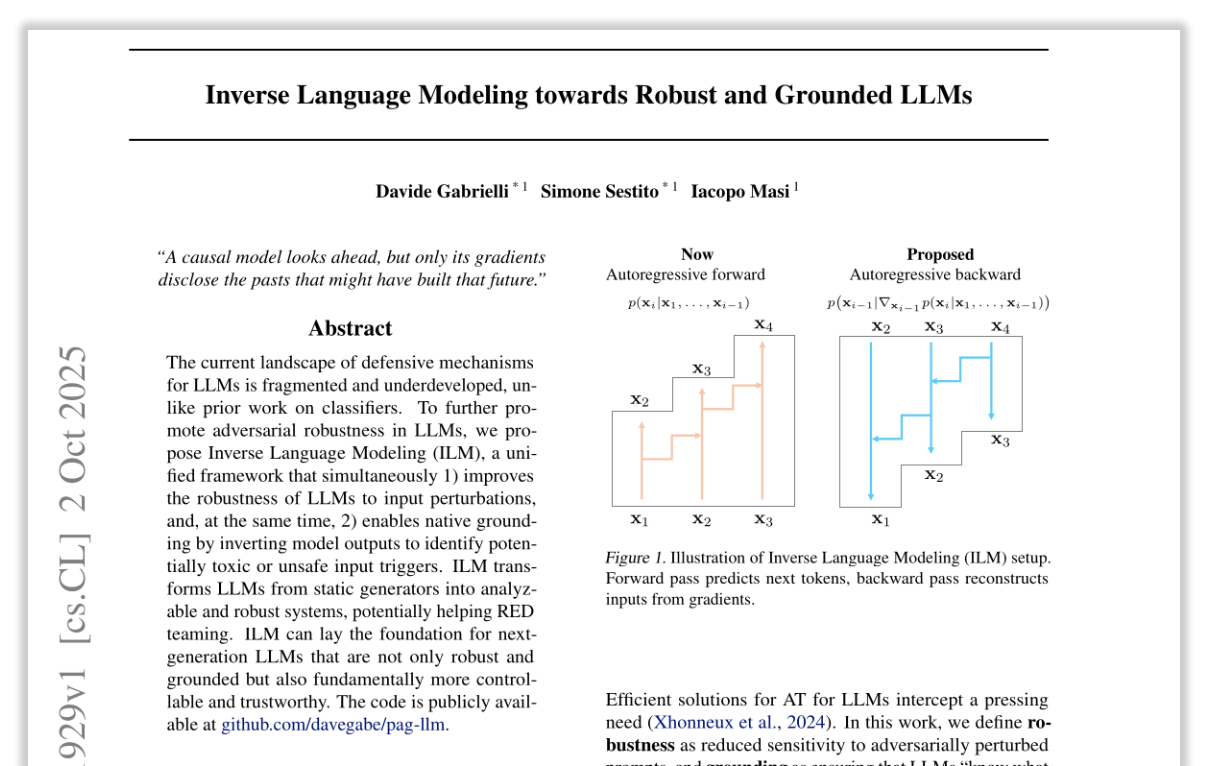
\includegraphics[height=0.8\pageheight]{assets/arxiv_paper.png}
\end{frame}

\backmatter
\end{document}
